\chapter{Continual Learning: An Overview}
\section{Introduction}
\textbf{Continual Learning} is motivated by the fact that human and other organisms has the ability to adapt, accumulate and exploit knowledge. A common setting for continual learning is to learn a sequence of contents one by one and behave as if they were observed simultaneously \citep{wang2023comprehensive}. Each task learned throughout the life time can be new skills, new examples of old skills, different environments, etc (Fig.\ref{fig:cl_1}, a). This attribute of continual learning makes it also referred to as \textbf{incremental learning} or \textbf{lifelong learning}.

Unlike conventional pipeline, where joint training is applied, continual learning is characterized by learning from dynamic data distributions. A major challenge is known as \textbf{catastrophic forgetting}, where \textit{adaptation to a new distribution generally results in a largely reduced ability to capture the old ones}. This dilemma is a facet of the trade-off between \textbf{learning plasticity} and \textbf{memory stability}: an excess of the former interferes with the latter, and vice versa. A good continual learning algorithm should obtain a strong \textbf{generalizability} to accommodate distribution differences within and between tasks (Fig.\ref{fig:cl_1}, b). As a naive baseline, retraining all old training samples (if allowed) makes it easy to address the above challenges, but creates huge computational and storage overheads (as well as potential privacy issues). In fact, continual learning is primarily intended to ensure \textbf{resource efficiency} of model updates, preferably close to learning only new training samples.

\begin{figure}[H]
    \centering
    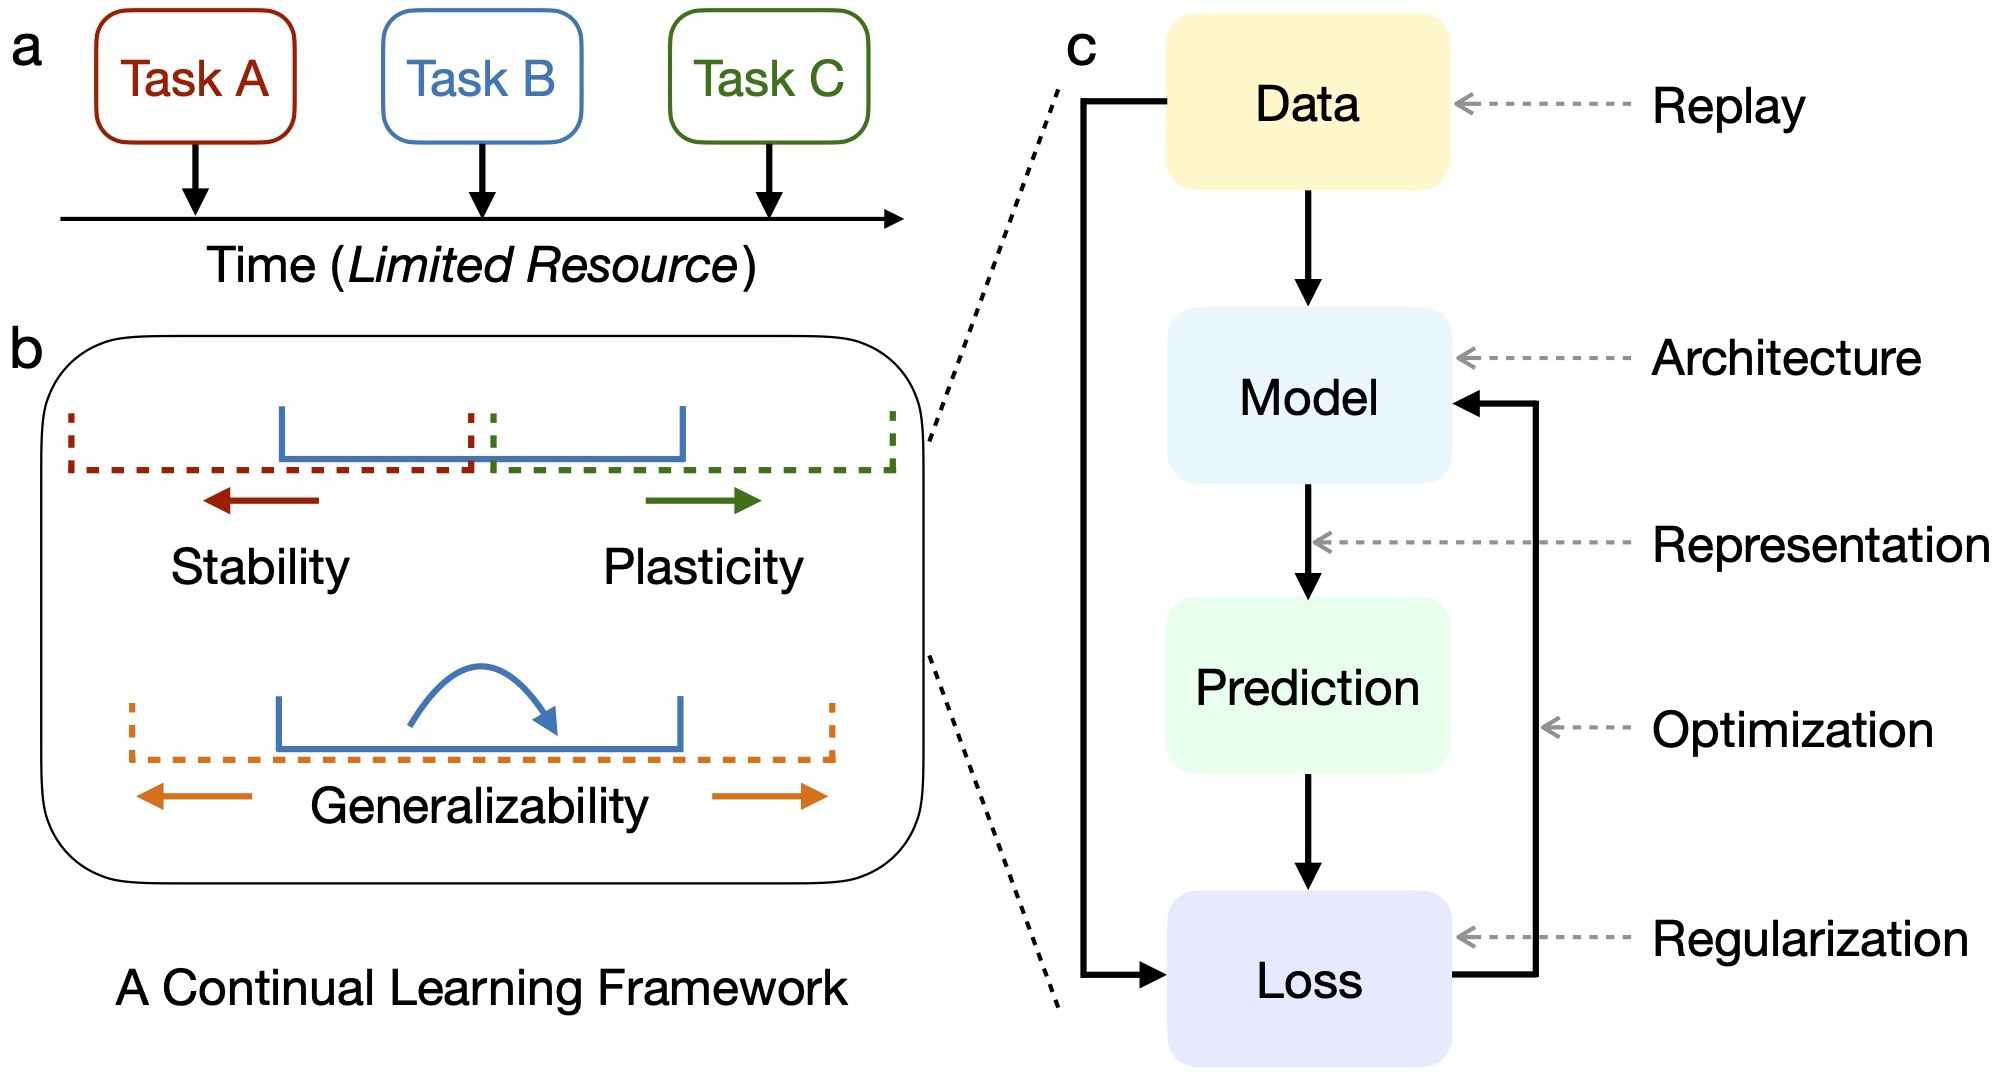
\includegraphics[width=0.7\linewidth]{imgs/continual_learning/cl_1.png}
    \caption{A conceptual framework of continual learning. \textbf{a}, Continual learning requires adapting to incremental tasks with dynamic data distributions. \textbf{b}, A desirable solution should ensure a proper balance between stability (red arrow) and plasticity (green arrow), as well as an adequate generalizability to intra-task (blue arrow) and inter-task (orange arrow) distribution differences. \textbf{c}, Representative strategies have targeted various aspects of machine learning.}
    \label{fig:cl_1}
\end{figure}

Numerous efforts have been devoted to addressing the above challenges, which can be conceptually separated into five groups (Fig.\ref{fig:cl_1}, c): \textit{regularization-based approach}; \textit{replay-based approach}; \textit{optimization-based approach}; \textit{representation-based approach}; and \textit{architecture-based approach}. These methods are \textit{closely connected}, e.g., regularization and replay ultimately act to rectify the gradient directions, and \textit{highly synergistic}, e.g., the efficacy of replay can be facilitated by distilling knowledge from the old model.

\section{Setup}
In this section, we first present a basic formulation of continual leanring. Then we introduce typical scenairos and evaluation metrics.

\subsection{Basic Formulation}
A continual learning model parameterized by \(\theta\) needs to learn corresponding task(s) with no or limited access to old training samples and perform well on their test sets. Formally, an incoming batch of training samples belonging to a task \(t\) can be represented as \(\mathcal{D}_{t, b}=\left\{\mathcal{X}_{t, b}, \mathcal{Y}_{t, b}\right\}\) where \(\mathcal{X}_{t, b}\) is the input data, \(\mathcal{Y}_{t, b}\) is the data label, \(t \in \mathcal{T}=\{1, \cdots, k\}\) is the task identity and \(b \in \mathcal{B}_{t}\) is the batch index ( \(\mathcal{T}\) and \(\mathcal{B}_{t}\) denote their space, respectively). Here we define a "task" by its training samples \(\mathcal{D}_{t}\) following the distribution \(\mathbb{D}_{t}:=p\left(\mathcal{X}_{t}, \mathcal{Y}_{t}\right)\left(\mathcal{D}_{t}\right.\) denotes the entire training set by omitting the batch index, likewise for \(\mathcal{X}_{t}\) and \(\left( \mathcal{Y}_{t}\right)\), and assume that there is no difference in distribution between training and testing. Under realistic constraints, the data label \(\mathcal{Y}_{t}\) and the task identity \(t\) might not be always available. In continual learning, the training samples of each task can arrive incrementally in batches (i.e., \(\left\{\left\{\mathcal{D}_{t, b}\right\}_{b \in \mathcal{B}_{t}}\right\}_{t \in \mathcal{T}}\) ) or simultaneously (i.e.,\(\left\{\mathcal{D}_{t}\right\}_{t \in \mathcal{T}}\)).

\begin{table}[H]
    \centering
    \renewcommand{\arraystretch}{1.75}
    \resizebox{\textwidth}{!}{
        \begin{tabular}{c|c|c}
            \hline
            \textbf{Scenario} & \textbf{Training}                                                                                                                                                                                                                               & \textbf{Testing}                                                                                  \\
            \hline IIL        & \(\left\{\left\{\mathcal{D}_{t, b}, t\right\}_{b \in \mathcal{B}_{t}}\right\}_{t=j}\)                                                                                                                                                           & \(\left\{p\left(\mathcal{X}_{t}\right)\right\}_{t=j ; t}\) is not required                        \\
            \hline DIL        & \(\left\{\mathcal{D}_{t}, t\right\}_{t \in \mathcal{T}} ; p\left(\mathcal{X}_{i}\right) \neq p\left(\mathcal{X}_{j}\right)\) and \(\mathcal{Y}_{i}=\mathcal{Y}_{j}\) for \(i \neq j\)                                                           & \(\left\{p\left(\mathcal{X}_{t}\right)\right\}_{t \in \mathcal{T}}, t\) is not required           \\
            \hline TIL        & \(\left\{\mathcal{D}_{t}, t\right\}_{t \in \mathcal{T}} ; p\left(\mathcal{X}_{i}\right) \neq p\left(\mathcal{X}_{j}\right)\) and \(\mathcal{Y}_{i} \cap \mathcal{Y}_{j}=\emptyset\) for \(i \neq j\)                                            & \(\left\{p\left(\mathcal{X}_{t}\right)\right\}_{t \in \mathcal{T} ; t}\) is available             \\
            \hline CIL        & \(\left\{\mathcal{D}_{t}, t\right\}_{t \in \mathcal{T}} ; p\left(\mathcal{X}_{i}\right) \neq p\left(\mathcal{X}_{j}\right)\) and \(\mathcal{Y}_{i} \cap \mathcal{Y}_{j}=\emptyset\) for \(i \neq j\)                                            & \(\left\{p\left(\mathcal{X}_{t}\right)\right\}_{t \in \mathcal{T} ; t}\) is unavailable           \\
            \hline TFCL       & \(\left\{\left\{\mathcal{D}_{t, b}\right\}_{b \in \mathcal{B}_{t}}\right\}_{t \in \mathcal{T}} ; p\left(\mathcal{X}_{i}\right) \neq p\left(\mathcal{X}_{j}\right)\) and \(\mathcal{Y}_{i} \cap \mathcal{Y}_{j}=\emptyset\) for \(i \neq j\)     & \(\left\{p\left(\mathcal{X}_{t}\right)\right\}_{t \in \mathcal{T}} ; t\) is optionally available  \\ \hline OCL  & \(\left\{\left\{\mathcal{D}_{t, b}\right\}_{b \in \mathcal{B}_{t}}\right\}_{t \in \mathcal{T}},|b|=1 ; p\left(\mathcal{X}_{i}\right) \neq p\left(\mathcal{X}_{j}\right)\) and \(\mathcal{Y}_{i} \cap \mathcal{Y}_{j}=\emptyset\) for \(i \neq j\) & \(\left\{p\left(\mathcal{X}_{t}\right)\right\}_{t \in \mathcal{T}} ; t\) is optionally available \\
            \hline BBCL       & \(\left\{\mathcal{D}_{t}, t\right\}_{t \in \mathcal{T}} ; p\left(\mathcal{X}_{i}\right) \neq p\left(\mathcal{X}_{j}\right), \mathcal{Y}_{i} \neq \mathcal{Y}_{j}\) and \(\mathcal{Y}_{i} \cap \mathcal{Y}_{j} \neq \emptyset\) for \(i \neq j\) & \(\left\{p\left(\mathcal{X}_{t}\right)\right\}_{t \in \mathcal{T} ; t \text { is unavailable }}\) \\
            \hline CPT        & \(\left\{\mathcal{D}_{t}^{p t}, t\right\}_{t \in \mathcal{T} p t}\), followed by a downstream task \(j\)                                                                                                                                        & \(\left\{p\left(\mathcal{X}_{t}\right)\right\}_{t=j ; t}\) is not required                        \\
            \hline\end{tabular}}
    \caption{A formal comparison of typical continual learning scenarios. \(\mathcal{D}_{t, b}:\) the training samples of task \(t\) and batch \(b\). \(|b|:\) the size of batch \(b\). \(\mathcal{B}_{t}:\) the space of incremental batches belonging to task \(t\). \(\mathcal{D}_{t}:\) the training set of task \(t\) (further specified as \(\mathcal{D}_{t}^{p t}\) for pre-training). \(\mathcal{T}:\) the space of all incremental tasks (further specified as \(\mathcal{T}^{p t}\) for pre-training). \(\mathcal{X}_{t}:\) the input data in \(\mathcal{D}_{t}\), \(p\left(\mathcal{X}_{t}\right):\) the distribution of \(\mathcal{X}_{t} . \mathcal{Y}_{t}:\) the data label of \(\mathcal{X}_{t}\).}
    \label{table:4.1}
\end{table}

\subsection{Typical Scenairo}

Detail of some tyical continual learning scenairos (refer to Table \ref{table:4.1} for a formal comparision):
\begin{itemize}
    \item \textit{Instance-Incremental Learning} (IIL): All training samples belong to the same task and arrive in batches.
    \item \textit{Domain-Incremental Learning} (DIL): Tasks have the same data label space but different input distributions. Task identities are not required.
    \item \textbf{\textit{Task-Incremental Learning}} (TIL): Tasks have disjoint data label spaces. Task identities are provided in both training and testing.
    \item \textbf{\textit{Class-Incremental Learning}} (CIL): Tasks have disjoint data label spaces. Task identities are only provided in training.
    \item \textit{Task-free Continual Learning} (TFCL): Tasks have disjoint data label spaces. Task identities are not provided in either training or testing.
    \item \textit{Online Continual Learning} (OCL): Tasks have disjoint data label spaces. Training samples for each task arrive as a one-pass data stream.
    \item \textit{Blurred Boundary Continual Learning} (BBCL): Task boundaries are blurred, characterized by distinct but overlapping data label spaces.
    \item \textit{Continual Pre-training} (CPT): Pre-training data arrives in sequence. The goal is to improve the performance of learning downstream tasks.
\end{itemize}

Lots of the above mentioned scenairo is messy, hence we will focus on the most popular scenairos: Task-Incremental Learning and Class-Incremental Learning.

\subsection{Evaluation Metrics}
\textbf{Overall performance} is typically evaluated by \textit{average accuracy} (AA) and \textit{average incremental accuracy} (AIA). Let \(a_{k, j} \in[0,1]\) denote the classification accuracy evaluated on the test set of the \(j\)-th task after incremental learning of the \(k\)-th task \((j \leq k)\). The output space to compute \(a_{k, j}\) consists of the classes in either \(\mathcal{Y}_{j}\) or \(\cup_{i=1}^{k} \mathcal{Y}_{i}\),  corresponding to the use of multi-head evaluation (e.g., TIL) or single-head evaluation (e.g., CIL). The two metrics at the \(k\)-th task are then defined as
\begin{equation*}
    \mathrm{AA}_{k}=\frac{1}{k} \sum_{j=1}^{k} a_{k, j}
\end{equation*}
AA represnets the overall performance at the current moment.

\begin{equation*}
    \mathrm{AIA}_{k}=\frac{1}{k} \sum_{i=1}^{k} \mathrm{AA}_{i}
\end{equation*}
AIA reflects the historical variaion.

\textbf{Memory stability} can be evaluted by \textit{forgetting measure} (FM) and \textit{backward transfer} (BWT). As for the former, the forgetting of a task is calculated by the difference between its maximum performance obtained in the past and its current performance:
\begin{equation*}
    f_{j, k}=\max _{i \in\{1, \ldots, k-1\}}\left(a_{i, j}-a_{k, j}\right), \forall j<k
\end{equation*}
FM at the \(k\)-th task is the average forgetting of all old tasks:
$$
    \mathrm{FM}_{k}=\frac{1}{k-1} \sum_{j=1}^{k-1} f_{j, k},
$$
As for the latter, BWT evaluates the average influence of learning the \(k\)-th task on all old tasks:
$$
    \mathrm{FWT}_{k}=\frac{1}{k-1} \sum_{j=2}^{k}\left(a_{j, j}-\tilde{a}_{j}\right),
$$
where the forgetting is usally reflected as a negative BWT.

\textbf{Learning plasticity} can be evaluated by \textit{intransience measure} (IM) and \textit{forward transfer} (FWT). IM is defined as the inability of a model to learn new tasks, calculated by the difference of a task between its joint training performance and continual leanring performance:
$$
    \mathrm{IM}_{k}=a_{k}^{*}-a_{k, k}
$$
where \(a_{k}^{*}\) is the classification accuracy of a randomly-initialized reference model jointly trained with \(\cup_{j=1}^{k} \mathcal{D}_{j}\) for the \(k\)-th task. In comparison, FWT evaluates the average influence of all old tasks on the current \(k\)-th task:
$$
    \mathrm{FWT}_{k}=\frac{1}{k-1} \sum_{j=2}^{k}\left(a_{j, j}-\tilde{a}_{j}\right)
$$
where \(\tilde{a}_{j}\) is the classification accuracy of a randomly-initialized reference model trained with \(\mathcal{D}_{j}\) for the \(j\)-th task.

\section{Method}

In this section, we go through representative continual learning methods.

\subsection{Regularization-based Aprroach}
This direction is characterized by adding explicit regularization terms to balance the old and new tasks, which usually requires storing a frozen copy of the old model for reference (Fig. \ref{cl_2}). Depending on the target of regularization, such methods can be divided into two sub-directions.

\begin{figure}[H]
    \centering
    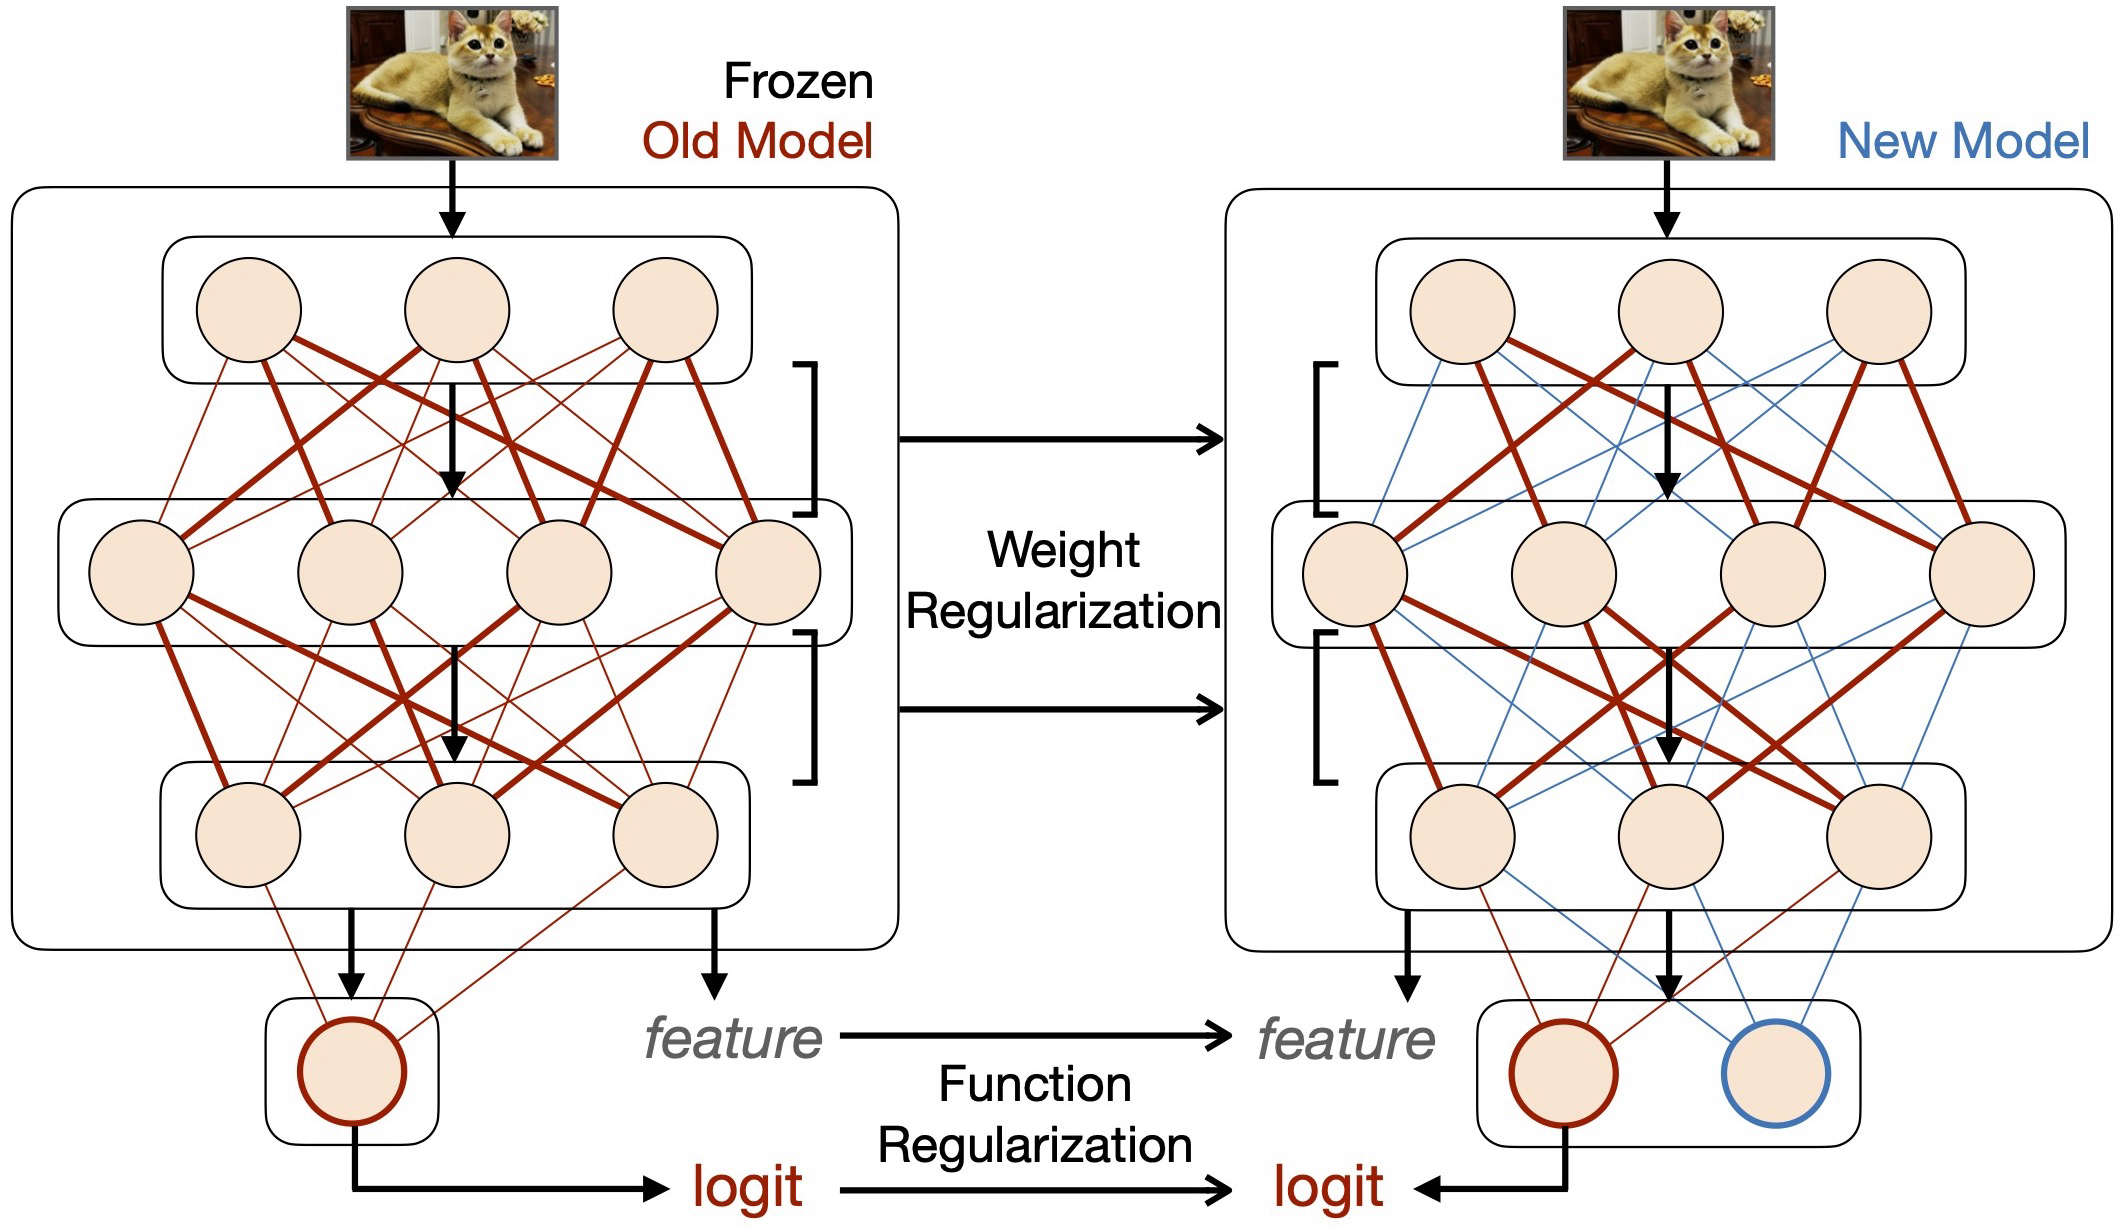
\includegraphics[width=0.7\linewidth]{imgs/continual_learning/cl_2.png}
    \caption{Regularization-based approach. This direction is characterized by adding explicit regularization terms to mimic the parameters (weight regularization) or behaviors (function regularization) of the old model.}
    \label{cl_2}
\end{figure}

The first is \textbf{weight regularization}, which selectively regularizes the variation of network parameters. A typical implementation is to add a quadratic penalty in loss function that penalizes the variation of each parameter depending on its contribution or ``importance'' to performing the old tasks, in a form originally derived from online Laplace approximation of the posterior under the Bayesian framework. The importance can be calculated by the Fisher information matrix (FIM), such as EWC. Numerous efforts have been devoted to designing a better imoportance measurement. SI online approximate the importance of each parameter by its contribution to the total loss vaiation and its update length over the entire training trajectory. MAS accumulates the importance measurements based on the sensitivity of predictive results to parameter changes, which is both online and unsupervised. RWalk combines regularization terms of SI and EWC to integrate their advantages.These importance measurements have been shown to be all tantamount to an approximation of the FIM, although stemming from different motivations.

There are also several works refining the implementation of the quadratic penalty.Since the diagonal approaximation of the FIM in EWC might lose information about the old tasks, R-EWC performs a factorized rotation of the parameter space to diagonalize the FIM. XK-FAC further considers the inter-example relations in approximating the FIM to better accommodate batch normalization. Observing the asymmetric effect of parameter changes on old tasks, ALASSO designs an asymmetric quadratic penalty with one of its sides overestimated.

Compared to learning each task within the constraints of the old model, which typically exacerbates the intransience, an \textit{expansion-renormalization} process of obtaining separately the new task solution and renormalizing it with the old model has shown to provide a better stability-plasticity trade off.

The second is \textbf{functional regularization}, which targets the intermediate or final output of the prediction function. This strategy typically employs the previously-learned model as the teacher and the currently-trained model as the student, while implementing knowledge distillation (KD) to mitigate catastrophic forgetting.

\subsection{Replay-based Approach}
We group the methods for approximating and recovering old data distributions into this direction (Fig. \ref{cl_3}). Depending on the content of replay, these methods can be further divided into three sub-directions, each with its own targets and challenges.

\begin{figure}[H]
    \centering
    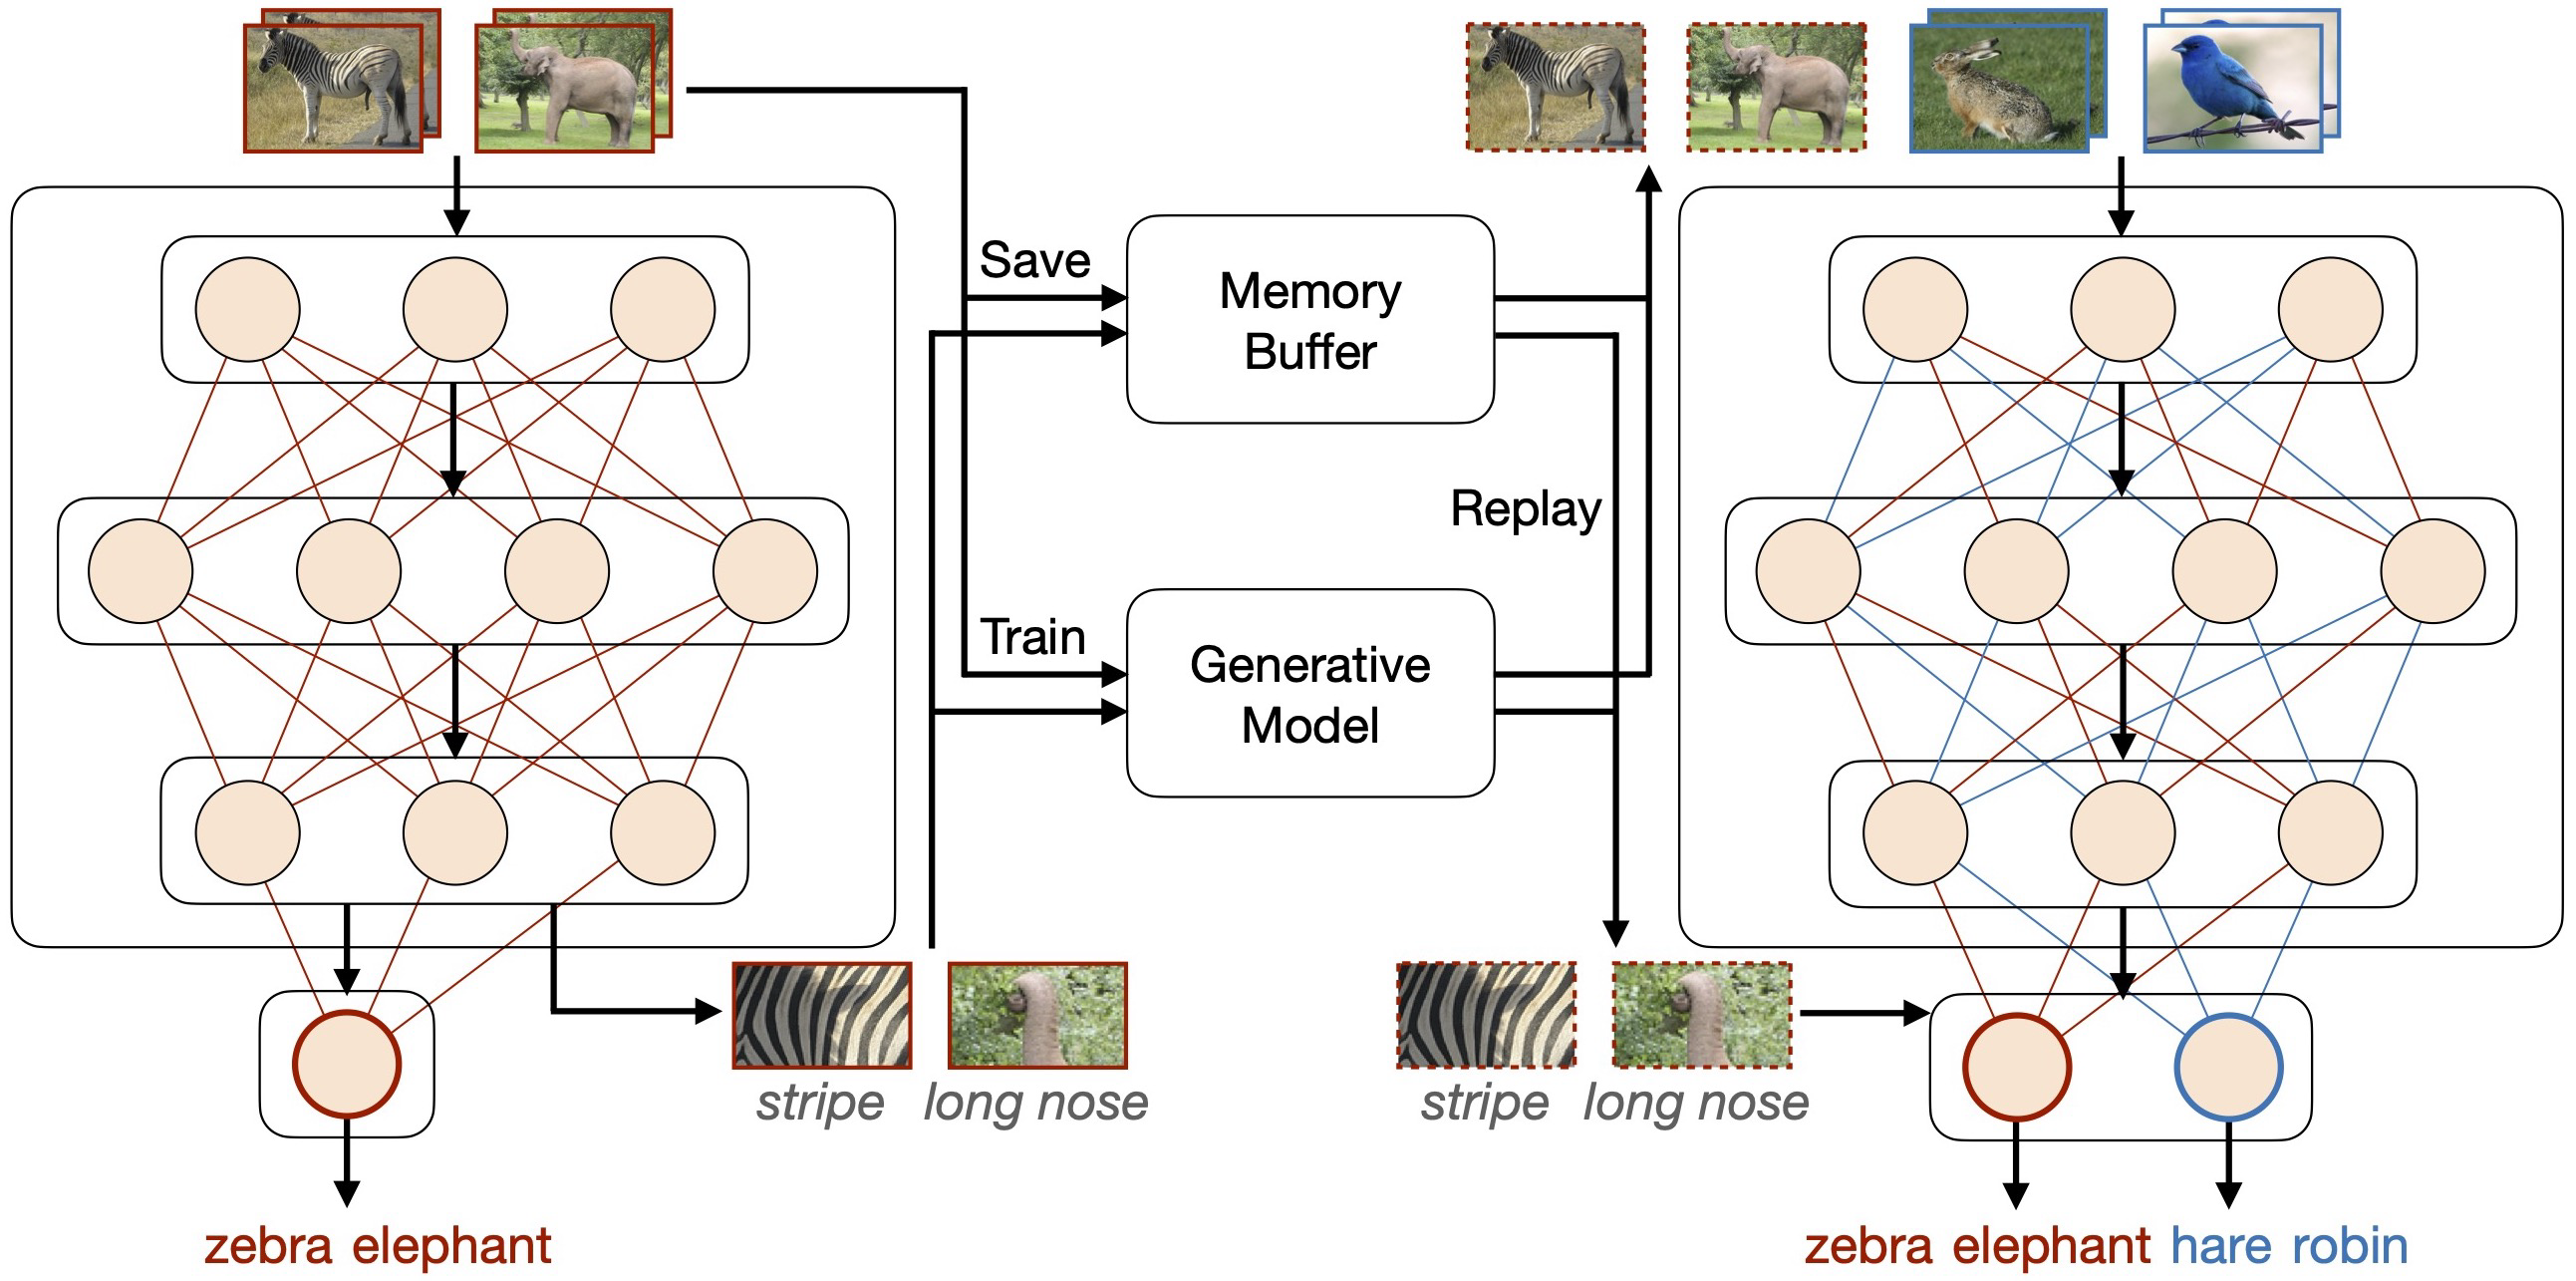
\includegraphics[width=0.7\linewidth]{imgs/continual_learning/cl_3.png}
    \caption{Replay-based approach. This direction is characterized by approximating and recovering the old data distributions. Typical subdirections include experience replay, which saves a few old training samples in a memory buffer; generative replay, which trains a generative model to provide generated samples; and feature replay, which recovers the distribution of old features through saving prototypes, saving statistical information or training a generative model.}
    \label{cl_3}
\end{figure}

The first is \textbf{experience replay}, which typically stores a few old training samples within a small memory buffer. Due to the extremely limited storage space, the key challenges consist of \textit{how to construct} and \textit{how to exploit} the memory buffer.  As for construction, the preserved old training samples should be carefully selected, compressed, augmented and updated, in order to recover adaptively the past information.  Some notable sampling methods are \textit{reservoir sampling} where randomly preserves a fixed number of old training samples obtained from each training batch and \textit{ring buffer} ensures an equal number of old training samples per class.  \textit{Mean-of-Feature} selects an equal number of old training samples that are closest to the feature mean of each class.  For exploitation, experience replay requires an adequate use of the memory buffer to recover the past information.  First, the effect of old training samples in optimization can be constrained to avoid catastrophic forgetting and facilitate knowledge transfer.  On the other hand, experience replay can be naturally combined with \textit{knowledge distillation} (KD), which additionally incorporates the past information from the old model.

The second is \textbf{generative replay} or pseudo-rehearsal, which usually requires training on additional generative model to replay generated data. This is closely related to continual learning of generative models themselves, as they also require incremental updates.

\subsection{Optimization-based Approach}
Continual learning can be achieved not only by adding additional terms to the loss function (e.g., regularization and replay), but also by explicitly designing and manipulating the optimization programs. A typical idea is to perform \textbf{gradient projection}.  A typical idea is to perform \textbf{gradient projection}. Some replay-based approaches as GEM, A-GEM, LOGD and MER constrain parameter updates to align with the direction of experience replay, corresponding to preserving the previous input space and gradient space with some old training samples. 